
\section{Data Collection}
\label{sec:datacollection}
In this section, we %first 
present our subject systems %. Then we present 
and our approach to collect performance regressions and configuration data.% related to system configuration.


\subsection{Subject Systems}
In this paper, we consider %We choose two open-source systems, 
\emph{Hadoop} and \emph{Cassandra} as two %the 
subject systems. % of our case study. 
\emph{Hadoop}~\cite{hadoop2012:White} is a distributed system infrastructure, whereas %. \med{do we need to advertise for hadoop in the following sentence? :)}\emph{Hadoop} performs data processing in a reliable, efficient, high fault tolerance, low cost and scalable manner. 
\emph{Cassandra} is a distributed NoSQL database management system. We choose these two subject systems since their performance is critical for the users and they have been studied in prior research on mining performance data~\cite{markASE,Chen:2014:DPA}. In addition, they have a large number of configuration options. The overview of our subject systems is shown in Table~\ref{tab:subject}.

\begin{table}[t]
  \centering
  %\tiny
  \caption{Our studied dataset.}%Overview of our subject systems.}
	\label{tab:subject}
    \begin{tabular}{|c|r|l|r|r|r|}
    \hline
    Subjects & \multicolumn{1}{c|}{\specialcell{\# Studied\\Releases}} & \multicolumn{1}{c|}{Last release} &  \multicolumn{1}{c|}{\# Commits} & \multicolumn{1}{c|}{\specialcell{\# Configuration\\Options}} & \multicolumn{1}{c|}{\# Tests} \\ \hline
    Hadoop & 7     & 2.7.3 & 803 & 365   & 1,853 \\ \hline
    Cassandra & 5     & 3.0.15 & 502 & 162   & 369 \\ \hline
    \end{tabular}
\end{table}


\subsection{Data Gathering}
To answer our research questions, we followed the approach that is summarized in Figure~\ref{fig:overview} and discussed below.
%In the subsection, we describe the pieces of data that we collected in order to answer our research questions. An overview of our data collection process is shown in Figure~\ref{fig:overview}. 

\begin{figure*}[t]
	\centering
		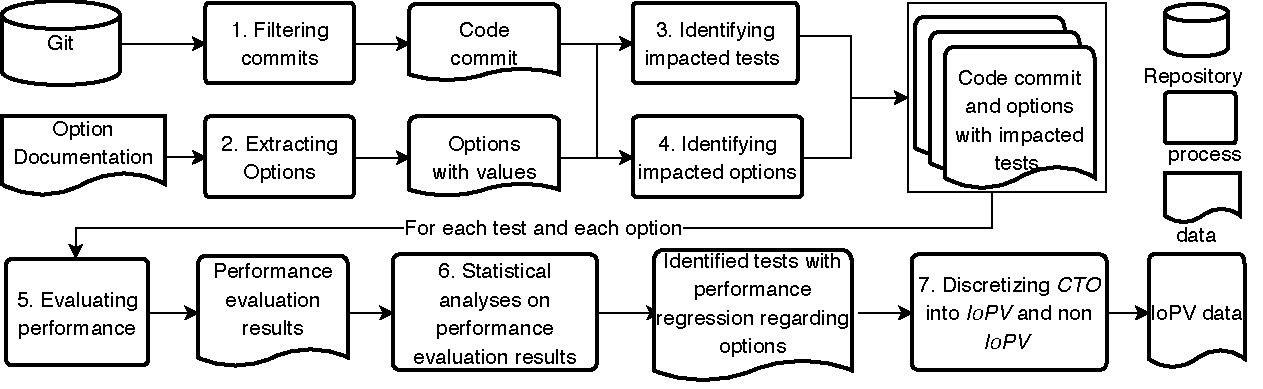
\includegraphics[width=.9\textwidth]{Figures/overview.pdf}
	\caption{An overview of our approach to collect data. \instance is a combination of Commit, a Test, and an Option.} %\bram{what is CTO?}} 
	\label{fig:overview} 
\end{figure*}

\subsubsection{Filtering Commits}

Since we study performance variation across different versions of a software system, we only consider source code related changes. In particular, we filter out commits without any \emph{java} source code changes. % after cloning the Git repositories. 
Furthermore, %multiple commits might be associated with the same feature or issue. In particular, 
developers can commit multiple changes toward fixing the same issue, which is defined in the issue tracking system. As \emph{Hadoop} and \emph{Cassandra} use JIRA as issue tracking system and have an explicit mapping between commits and issues, we use the issue ID mentioned in the commit messages to identify the commits that belong to the same issue. If multiple commits are associated with the same issue, we only consider the last commit. This is important as developers can initially introduce a regression but then fix it before releasing the code changes related to the issue. %\bram{did we add this to threats section?}


%In the first step, we filter commits that only have source code changes. In particular, we clone our subject systems from Github repository. Then we checkout to each commit and use \emph{git log} command to list all the files that are changed in each commit. In our subject systems, we extract the commits that have source code changes changes to \emph{java} files. To accomplish one development task, multiple commits, including temporary commits, may be made. We would like to avoid considering such temporary commits. Since all our subject systems use JIRA as their issue tracking systems, we use the issue id mentioned in their commit messages to identify commits that belong to the same issue. If multiple commits are associated with the same issue, we only consider the last commit.

\subsubsection{Extracting Options}

In the second step, we extract configuration options and their corresponding values for each subject system (i.e., 355 and 162 configuration options in the last studied releases of \emph{Hadoop} and \emph{Cassandra}, respectively). %There exist hundreds of configuration options in \emph{Hadoop} and \emph{Cassandra}. In particular, there are 355 and 162 configuration options in the last release of \emph{Hadoop} and \emph{Cassandra}, respectively. 
We obtain option names and default values by crawling the documentation of \emph{Hadoop}\footnote{\url{https://hadoop.apache.org/docs/current/hadoop-project-dist/hadoop-common/core-default.xml}} and \emph{Cassandra}\footnote{\url{https://cassandra.apache.org/doc/latest/configuration}}, by and extracting the configuration file that is shipped with the project's releases. Finally, we manually classified the extracted options based on their expected data types (e.g., Boolean when the default value is \emph{TRUE} or \emph{FALSE}).

%Therefore, to collect all the option names, we develop a crawler in Python to gather options from the official configuration website of \emph{Hadoop} and \emph{Cassandra}\footnote{\url{https://cassandra.apache.org/doc/latest/configuration}}.
%We also extract the type and values of options. For each option, we extract its default value and manually divide its type into boolean, numeric, and enumerated string. 
%For example, if we find that the default value of an option is \emph{FALSE}, we consider the type of such option to be boolean. 

\subsubsection{Identifying Impacted Tests}
\label{sec:impactedtests}
We automatically create a mapping between the changed source code in each commit and the existing unit tests. %%a mapping between the existing unit tests and %correspondingly 
%the changed source code for that commit. 
We derive such commit-test mapping based on the automatically generated method-level code coverage results, similar to our prior study~\cite{jinfu_tse2020}. %\bram{is this explained next?}
%\med{I see that the two sentences that describe the approach are commented, it looks like we are asking readers to read 2 papers to understand our approach. I still think that we should put it back}
%for each commit all the changed methods % by adding invocation to logging libraries 
%and run all the exiting unit tests. The tests that run the instrumented source code are the test that are associated with a commit's change. 
%\heng{Check if the following is right: } 
For each commit, we automatically add logging instrumentation to each method that will print log messages that indicate the execution of the method at runtime\footnote{Note that the instrumented versions are only used to identify impacted tests and options, and they are not used in our actual performance evaluation.}.
We then run each test for the commit. A test is considered impacted by the commit if any instrumented logging is output.
Afterwards, we only run the tests that execute the changed source code for a given commit since executing all the existing tests of a software system for each commit and each possible configuration is practically infeasible. In addition, running those tests that are not impacted by the code change of a commit is not likely to detect performance variations (regressions or improvements under some values of an option). 

%in every version of the source code of our subject systems by adding invocation to logging libraries. We run all the available tests of each released version of the subject systems. By analyzing the output of our instrumentation, we obtain a list of methods that are executed during the running of each test. Then, we can create mappings between each test and the executed methods of the test. With such a mapping between tests and methods in the source code, for each commit, we can identify the tests that are likely to be impacted by identifying the methods that are changed in the commit, i.e., a method-to-test mapping for each commit. Due to the resources needed for creating such mappings, we only update such mappings for every release of the subject systems.

%We consider using all the functional test that exist in the repository. We use these tests since these tests are maintained and typically executed regularly during every build in the release pipeline of software development~\cite{DBLP:journals/software/TillmannS06}. Not all the tests are impacted by the code changes and options in a commit and running those un-impacted tests is not likely to detect performance regressions. 

%To identify all the impacted tests by each commit, we create mappings between source code and tests. We automatically instrument all the methods in every version of the source code of our subject systems by adding invocation to logging libraries. We run all the available tests of each released version of the subject systems. By analyzing the output of our instrumentation, we obtain a list of methods that are executed during the running of each test. Then, we can create mappings between each test and the executed methods of the test. With such a mapping between tests and methods in the source code, for each commit, we can identify the tests that are likely to be impacted by identifying the methods that are changed in the commit, i.e., a method-to-test mapping for each commit. Due to the resources needed for creating such mappings, we only update such mappings for every release of the subject systems.

\subsubsection{Identifying Impacted Options}% \heng{Identifying Impacted Options?}}
Similar to identifying which tests to run for a given commit, we also select which configuration options to change when running each of those tests. To do so, we first identify how \emph{Hadoop} and \emph{Cassandra} access the value of a configuration option by searching for option names in the source code files. We found that all the options are accessible via \emph{getters} that are defined in one class provider (e.g., \emph{DatabaseDescriptor.java}\footnote{\url{https://github.com/apache/cassandra/blob/trunk/src/java/org/apache/cassandra/config/DatabaseDescriptor.java}} to access the \emph{Cassandra}'s options). Second, we identify the methods that invoke these configuration options' \emph{getters}. Finally, we dynamically identify which of these methods are executed when running a test similarly to the approach discussed in Section~\ref{sec:impactedtests}. If any method that can access an option is executed, the option is considered impacted by the commit.

%In this step, we identify the methods which call the options in direct or indirect ways. We call such methods impacted methods. We first extract the methods that call the options directly. We call such methods direct-call-method. To extract such direct-call-method, we follow a heuristic approach to find the methods that contain configuration names. In particular, we use ``grep -r option\_name *" to search all the methods that contain the option names in the path of each subject system. With the returned methods, we manually filter and determine the direct-call-methods. In our subject systems, we find that all the direct-call-methods are in the same \emph{Java} class file. For example, all the direct-call-methods are in the class named \emph{DatabaseDescriptor.java}\footnote{\url{https://github.com/apache/cassandra/blob/trunk/src/java/org/apache/cassandra/config/DatabaseDescriptor.java}}.

%Second, we extract the methods that call the direct-call-method. We iterate all the methods from the method-to-test mapping generated in last subsection, to find the methods that call the direct-call-method. Finally, based on the mapping between options and impacted methods, with mapping between methods and tests, we can generate the methods and tests impacted by each option.

\subsubsection{Evaluating Performance}
\label{evaluation}
After obtaining which tests and which options are impacted by each commit, we exercise the test on each commit and its parent commit (i.e., the previous commit) to evaluate their respective performances. %For each test, 
We first execute each test with all the configuration options set at their default values. Then, we alter the value of one configuration option at a time. For the configuration options with boolean values, we alter the configuration option to the value that is not the default. For example, if the default value is \emph{TRUE}, we would alter the value to be \emph{FALSE}. For numeric type option, we alter the configuration option once to the value that is double the default value and once to half of the default value. For example, if a configuration option has a default value of $100$, we would run the test altering the value to $200$, then run the same test altering the value to $50$. %\ian{I don't understand the next sentence.\med{is it better now?}}
For enumeration-typed options, we alter to each of the possible values.% for the enumerate type options. %For enumerated string type option, we execute the same test multiple times, each of which with one of the existing enumerated string values. %Note that we do not execute the tests with the instrumented source code that we discussed in Section~\ref{sec:impactedtests}. 

%We exercise the selected tests with different configurations of each pair of current and parent commits to evaluate their performance. In particular, we execute the same tests with same configuration option in different option values. In terms of different option values, for boolean type option, we execute the same test with \emph{TRUE} and \emph{FALSE} values. For numeric type option, we exetute the test with \emph{default}, 2*\emph{default}, and \emph{default}/2 values. For enumerated string type option, we execute the same test with all the existing enumerated string values.

Our performance evaluation environment uses the Google Compute Engine~\footnote{\url{https://cloud.google.com/compute}} with 8GB memory and 16 cores CPU. In order to generate statistically rigorous performance results, we adopt the practice of repetitive measurements~\cite{peterfse} to evaluate performance. Conservatively, we executed each test 30 times independently, which is larger than prior work that  %since prior research often only 
repeat a test only 5 to 20 times~\cite{Laaber2018MSR, Leitner2016TIT,DBLP:journals/ese/LaaberSL19}. 

To measure the performance that is associated with each test, we %catch the process of each test and 
use a performance monitoring tool named \emph{psutil}~\footnote{\url{https://github.com/giampaolo/psutil}} (Python system and process utilities). % to capture performance data of such process.
\emph{Psutil} can capture detailed performance metrics and has been widely used in prior research~\cite{DBLP:conf/icsm/ChenS17,DBLP:conf/wosp/YaoPSSTS18}. We collect both domain level and physical level performance metrics. In our execution, we collect five performance metrics during the execution, i.e., response time, CPU usage, memory usage, I/O read and I/O write.

The entire data collection process took around 12,536 machine-hours.

\subsubsection{Statistical Analyses on Performance Evaluation Results}
\label{sec:statisticalAnalysis}

To identify the \inconsistent, we statistically compare the performance of a given test and a configuration option value before and after each commit using the %We perform statistical analyses on the performance data from each pair of current and parent commits to determine the existence and the magnitude of performance regression in a statistically rigorous manner. 
%We use 
Mann-Whitney U test~\cite{nachar2008mann} %to examine if there exist statistically significant differences 
(i.e., $\alpha$ $=$ 0.05) and Cliff\textquotesingle s delta~\cite{ES2006:Becker}, which measures the magnitude of performance regressions. We choose Mann-Whitney U test since it does not have any assumption on the distribution of the data. Researchers have shown that reporting only the statistical significance may lead to erroneous results (i.e., if the sample size is very large, p-value can indicate statistical significance even if the difference is trivial). Thus, we also use Cliff\textquotesingle s delta to quantify the magnitude of the differences (a.k.a., effect sizes). Cliff\textquotesingle s delta measures the effect size statistically and has been used in prior engineering studies~\cite{ICSE2002:Kitchenham, Liao2020LogPerfReg, DBLP:journals/ese/LiCSH18}. Cliff\textquotesingle s delta ranges from -1 to +1, where a value of 0 indicates two identical distributions.

For each combination of commit, test and option value, we obtain a Cliff\textquotesingle s delta value. We then calculate the differences between the maximum and minimum Cliff\textquotesingle s delta for each option's different values, which the next subsection uses to categorize a combination of commit, test and option as \inconsistent or non-\inconsistent.%, as discussed in the following paragraph.

We also consider a test to be a performance regression when the value of the effect size is positive and has either medium ($0.33 <$ \emph{Cliff\textquotesingle s delta} $\leqslant 0.474$) or large ($0.474 < $\emph{Cliff\textquotesingle s delta}) magnitude. On the other hand, we consider a test to manifest a performance improvement if the value of the effect size is negative and has a medium ($-0.33 <$ \emph{Cliff\textquotesingle s delta} $\leqslant -0.474$) or large ($-0.474 > $\emph{Cliff\textquotesingle s delta}) magnitude. 

Note that we perform this statistical analysis for each performance metric (i.e., response time, CPU usage, memory usage, I/O read and I/O write) separately. For example, a commit may show a CPU regression or improvement, but not show any difference for the response time. 

%Based on the statistical analysis results, each commit is labelled with five different performance metrics (i.e., response time, CPU usage, memory usage, I/O read and I/O write) that are collected during the execution of the test. For example, the CPU label indicates whether the test demonstrate performance regression in terms of CPU usage. \ian{needs to say both regression and improvement}


\subsubsection{Discretizing \instance into \inconsistent and non-\inconsistent}
\label{sec:discretizing}
In the final step, we categorize each commit, test, and option (\instance) into \inconsistent or non-\inconsistent %the maximum difference values into \emph{small} and \emph{large} differences 
based on an automatically determined threshold. Our intuition is that the maximum difference values (a-b in Figure~\ref{fig:description}) would be concentrated in either small values %\bram{what values is this referring to?} 
(i.e., when adjusting a option does not make a difference) or large values (i.e., when adjusting a option does make a difference), which is demonstrated in Figure~\ref{fig:description}. % using the real data from Hadoop version.

Specifically, we use Ckmeans.1d.dp~\cite{Ckmeans138:online}, a one-dimensional clustering method, to find a threshold that separates the maximum difference values of all \emph{CTO}s %\bram{of all CTOs? or what is granularity of this clustering?} 
into two groups, i.e., \inconsistent and non-\inconsistent (see Figure~\ref{fig:threshold_hadoop} and ~\ref{fig:threshold_cassandra}). Note that the option variation ranges between 0, when there is no variation, and 2, when the effect size (cf. Section~\ref{sec:statisticalAnalysis}) is 1 for one option value and -1 for another value of the same option.

Most of the thresholds obtained using CKmeans.1d.dp are close to 1. This indicates, as an example, that one option value might show a large performance effect size compared to the prior commit, while another value for the same option does not show any difference from the prior commit (effect size equals to 0). A second example is when one option's value shows a large performance improvement over the prior commit (effect size equals to -1), when another value of the same option does not show any statistically significant difference (effect size equals to 0).
%The categorized difference values (i.e., \emph{small} or \emph{large}) is our target variable.

\begin{figure}[t]
	\centering
        \begin{subfigure}{0.19\textwidth}
                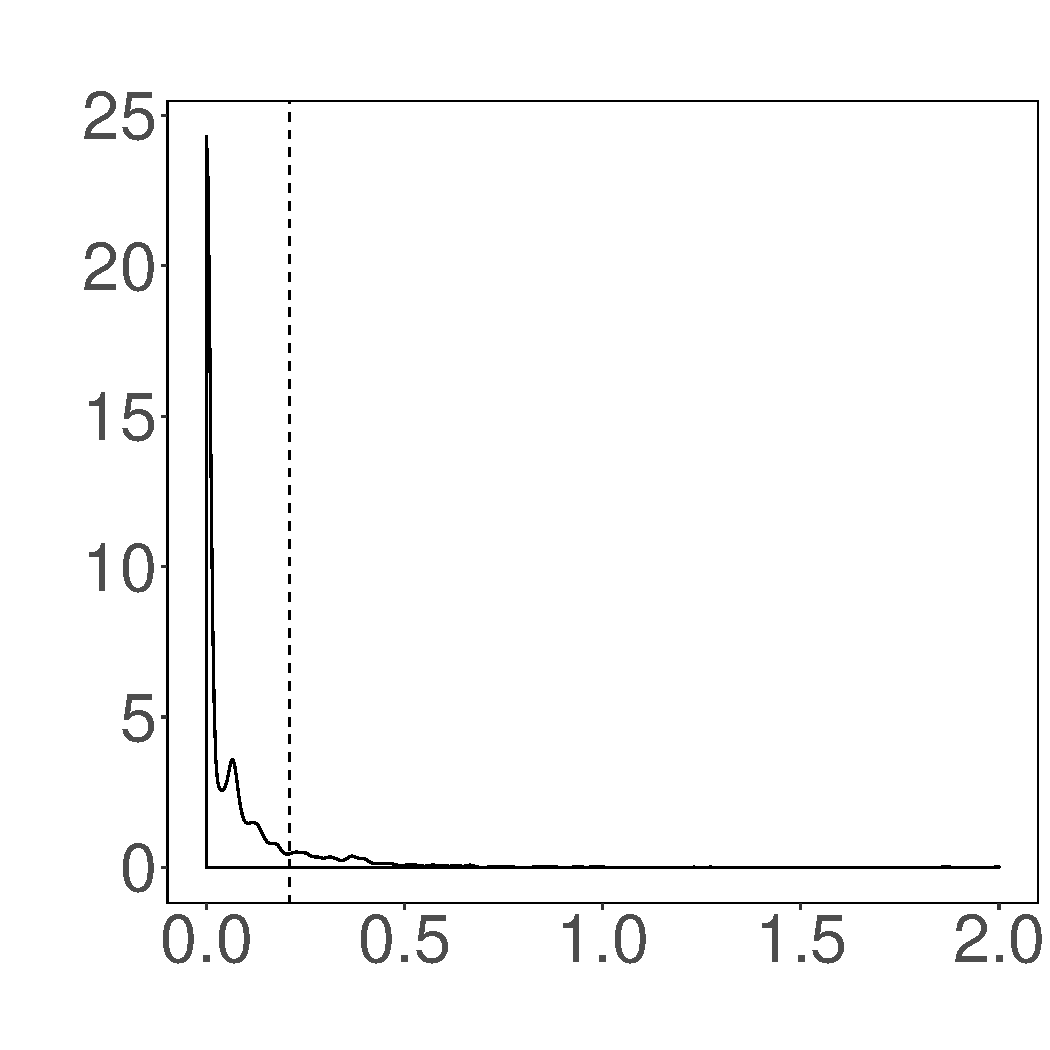
\includegraphics[width=\linewidth]{Figures/runtime-hadoop-cluster.pdf}
                \caption{Res. time}
        \end{subfigure}%
        \begin{subfigure}{0.19\textwidth}
                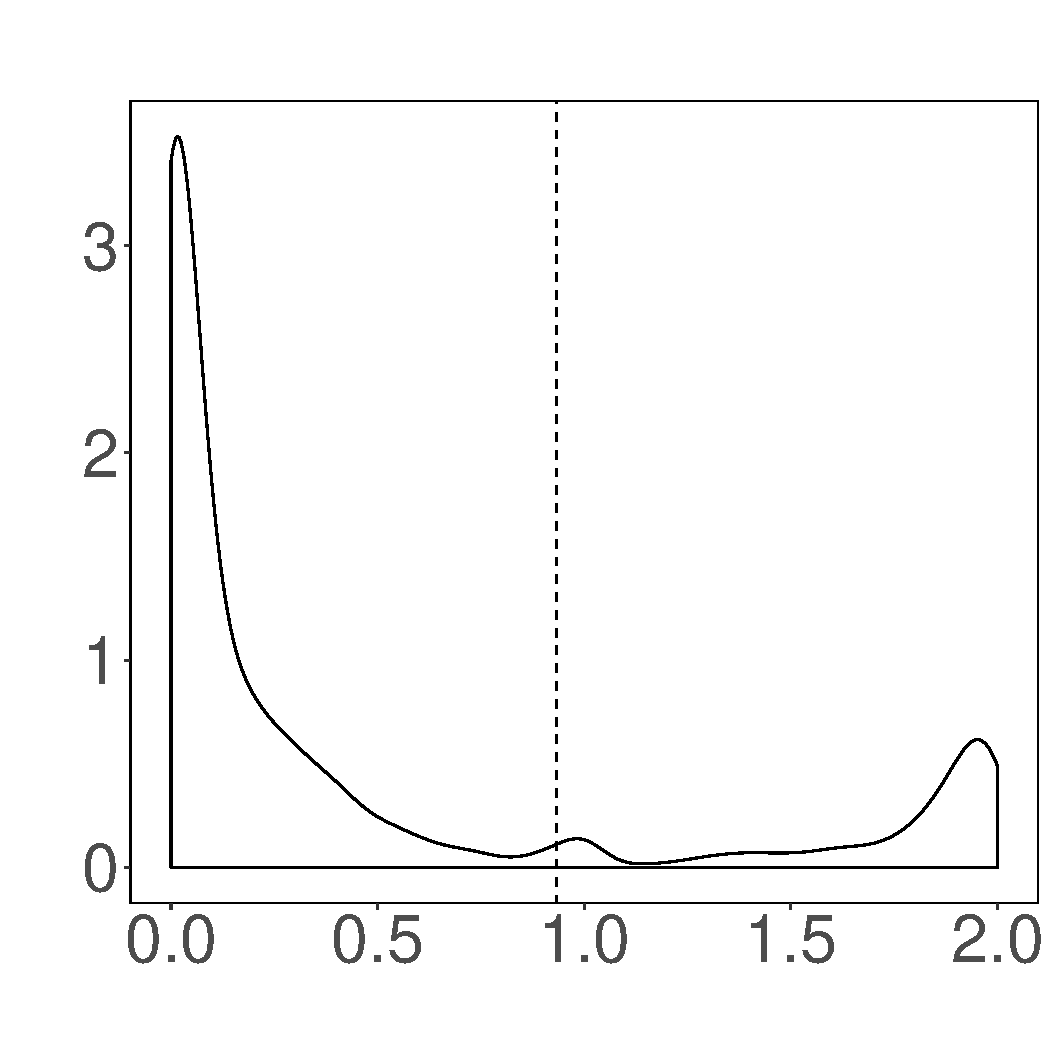
\includegraphics[width=\linewidth]{Figures/cpu-hadoop-cluster.pdf}
                \caption{CPU}
        \end{subfigure}%
        \begin{subfigure}{0.19\textwidth}
                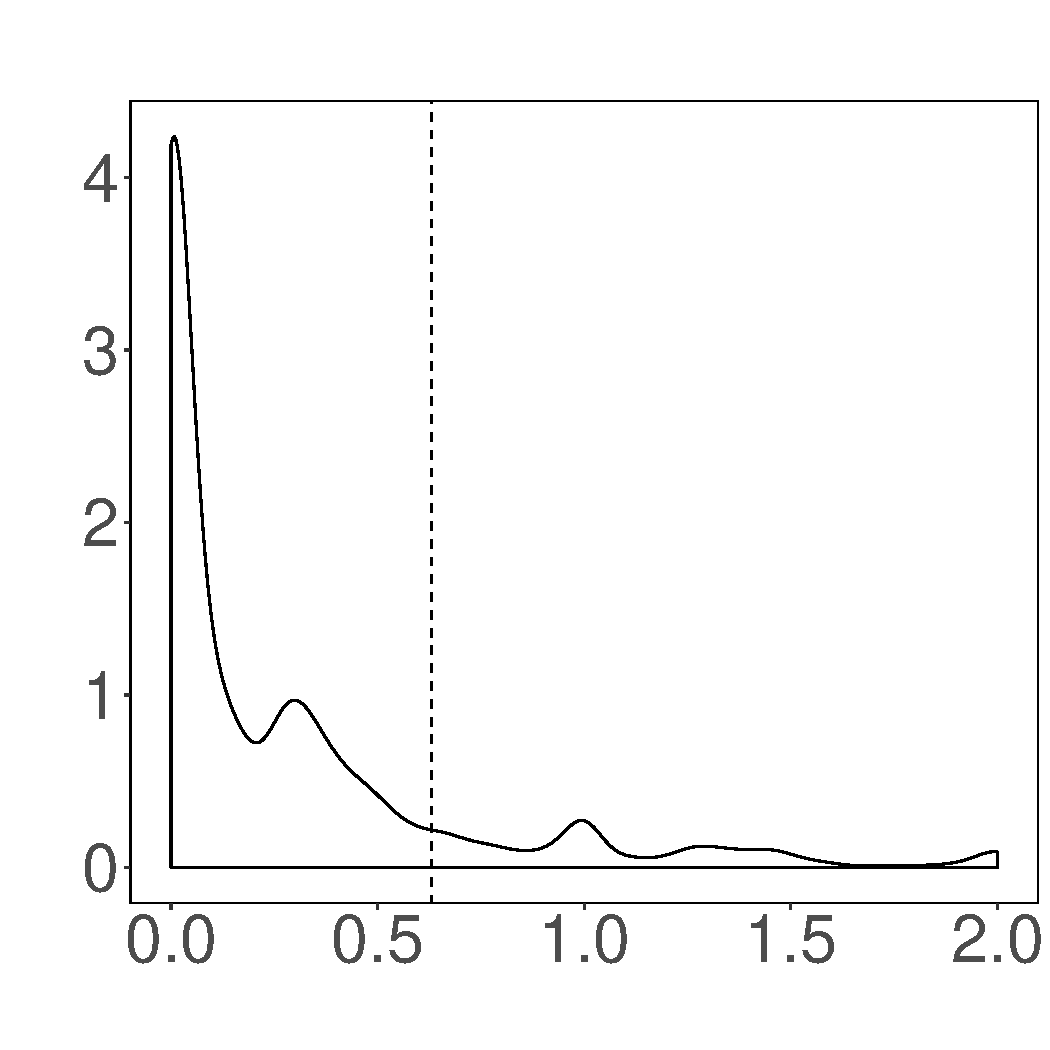
\includegraphics[width=\linewidth]{Figures/mem-hadoop-cluster.pdf}
                \caption{Memory}
        \end{subfigure}%
        \begin{subfigure}{0.19\textwidth}
                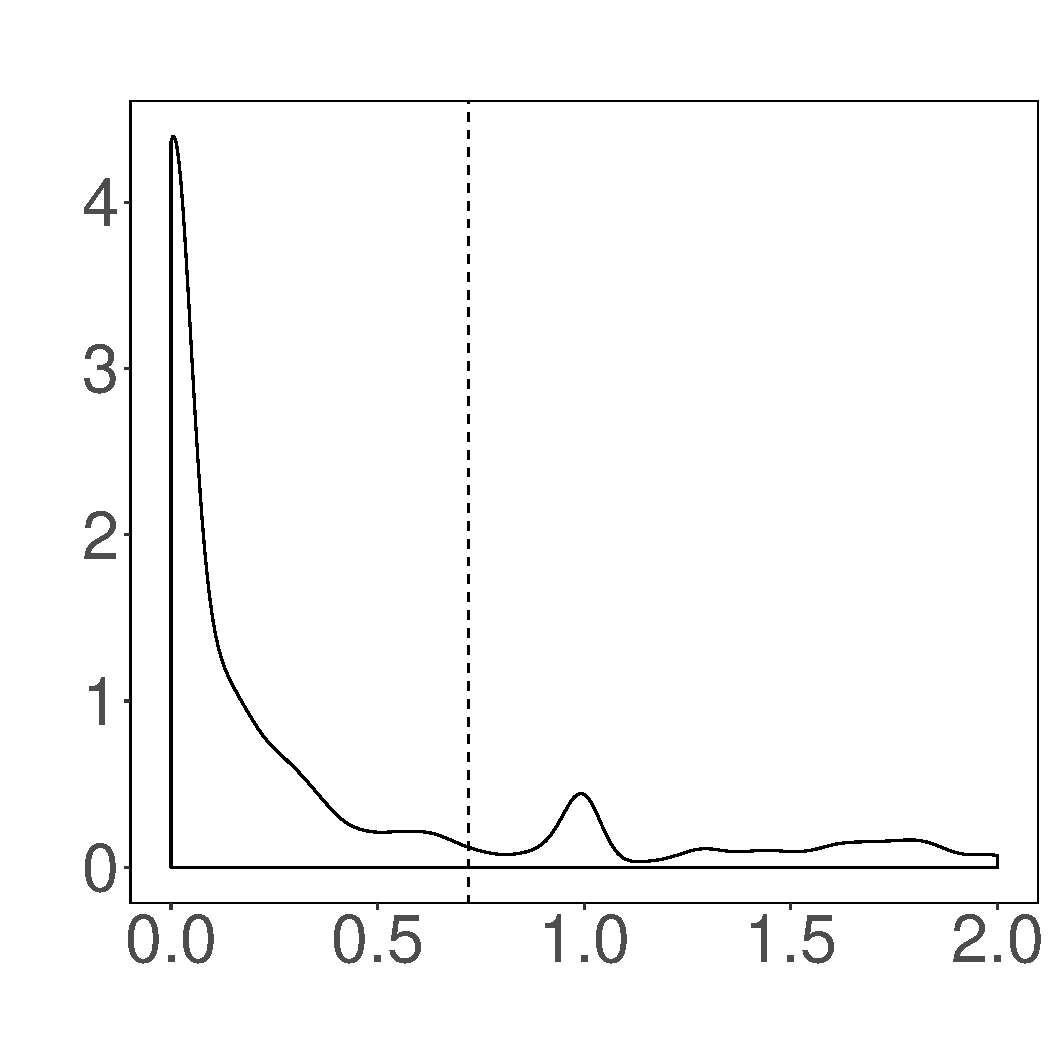
\includegraphics[width=\linewidth]{Figures/ioread-hadoop-cluster.pdf}
                \caption{I/O read}
        \end{subfigure}
        \begin{subfigure}{0.19\textwidth}
                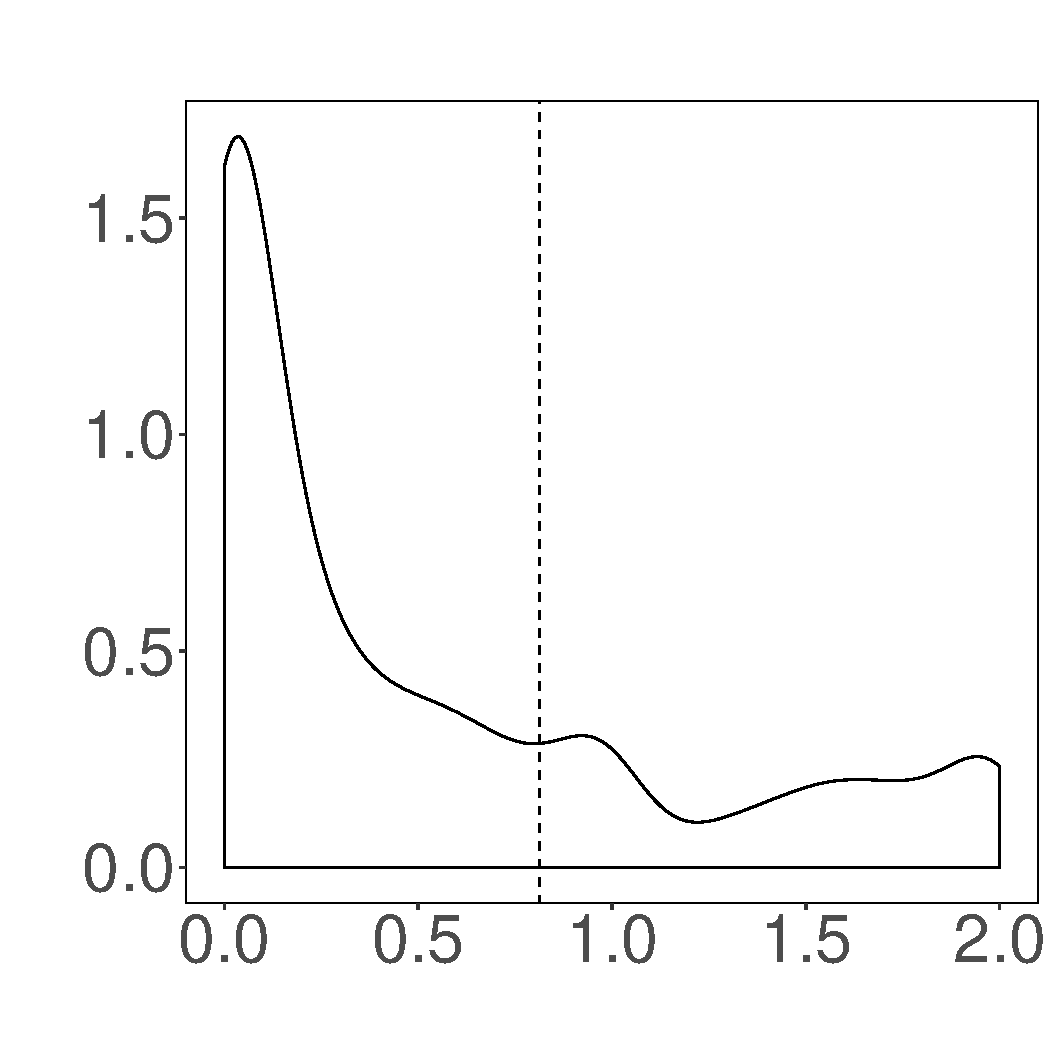
\includegraphics[width=\linewidth]{Figures/iowrite-hadoop-cluster.pdf}
                \caption{I/O write}
        \end{subfigure}
        
	\caption{The automatically obtained thresholds for splitting option variation into \inconsistent and non-\inconsistent groups for \emph{Hadoop}.} % \med{Canssadra or Hadoop? Both fig. 3 and fig. 4 showed Hadoop}.}
	\label{fig:threshold_hadoop}
% 	\vspace{-0.15cm}
\end{figure}

\begin{figure}[t]
	\centering
        \begin{subfigure}{0.19\textwidth}
                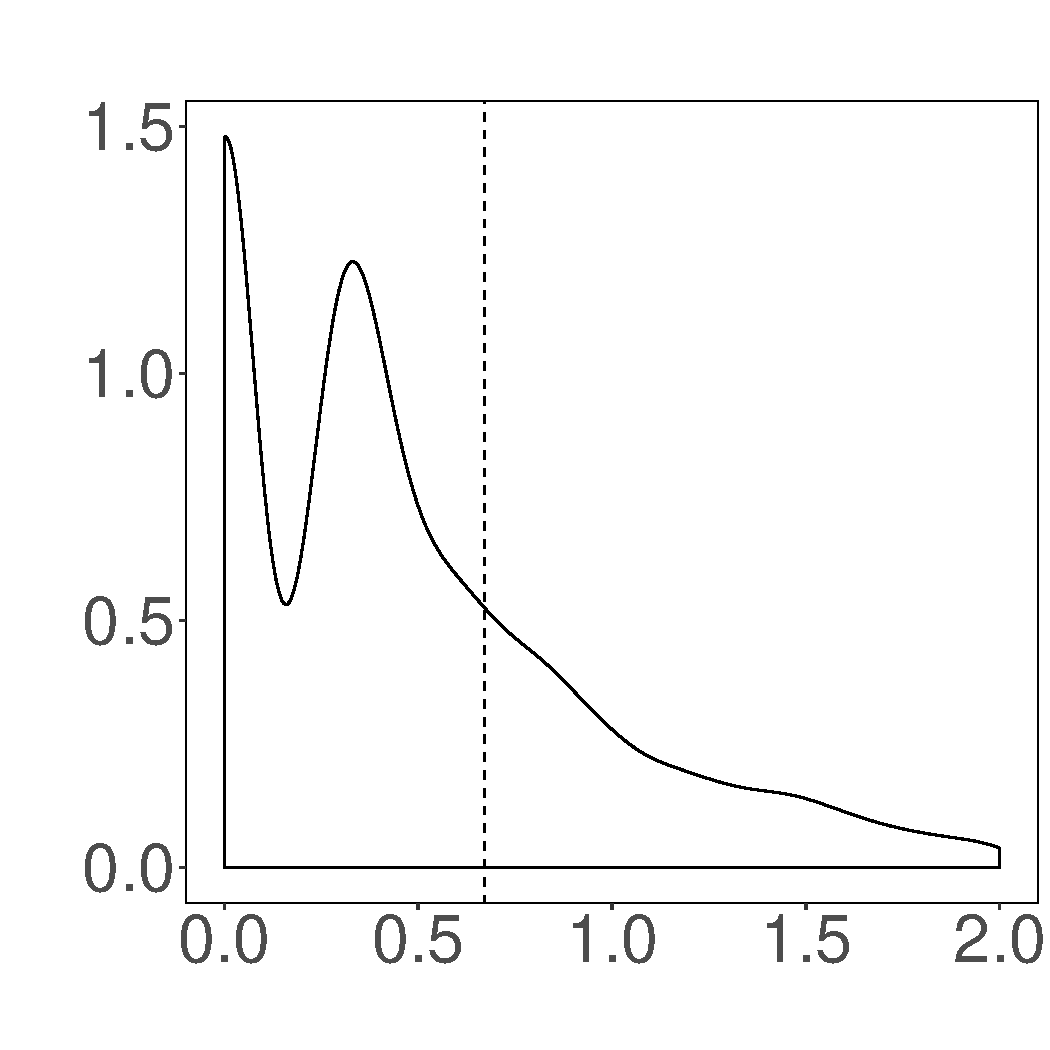
\includegraphics[width=\linewidth]{Figures/runtime-cassandra-cluster.pdf}
                \caption{Res. time}
        \end{subfigure}%
        \begin{subfigure}{0.19\textwidth}
                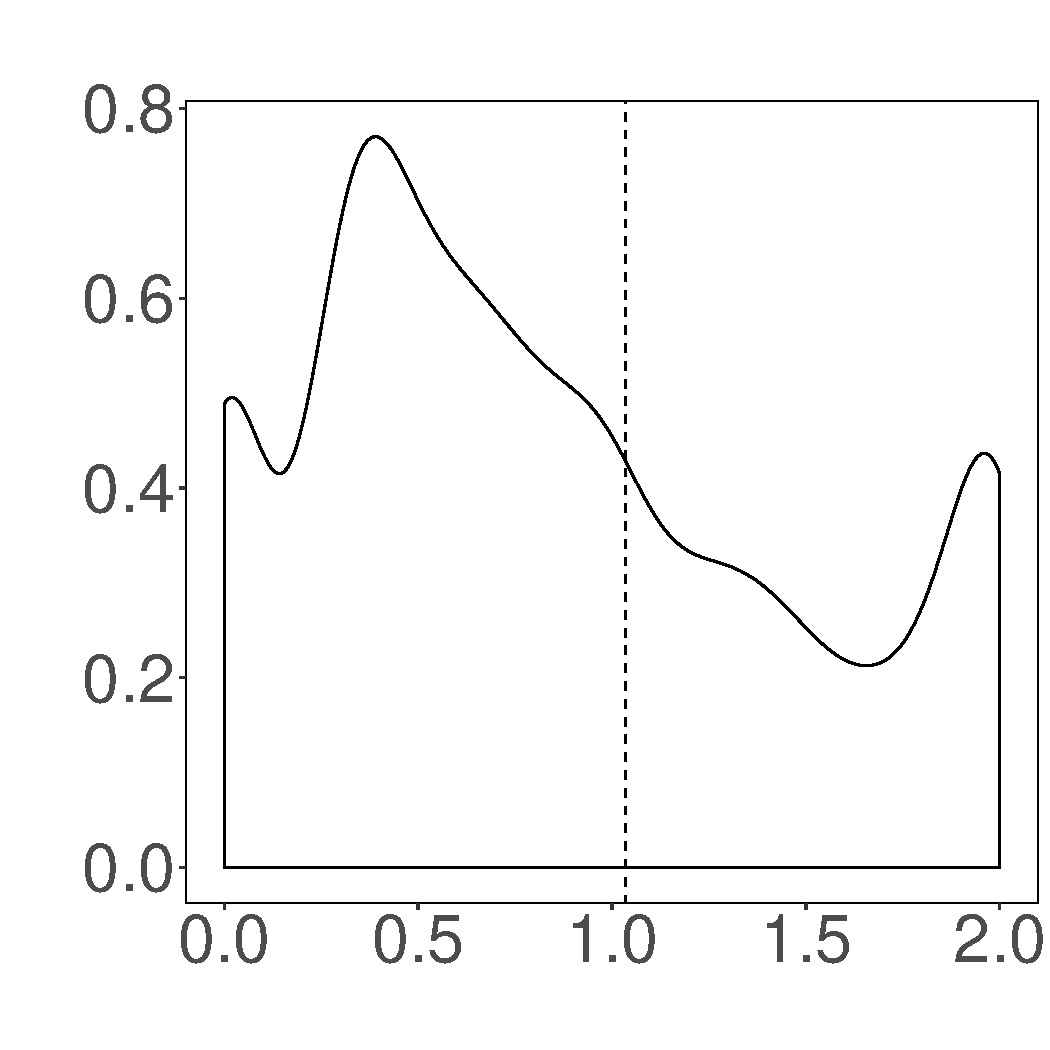
\includegraphics[width=\linewidth]{Figures/cpu-cassandra-cluster.pdf}
                \caption{CPU}
        \end{subfigure}%
        \begin{subfigure}{0.19\textwidth}
                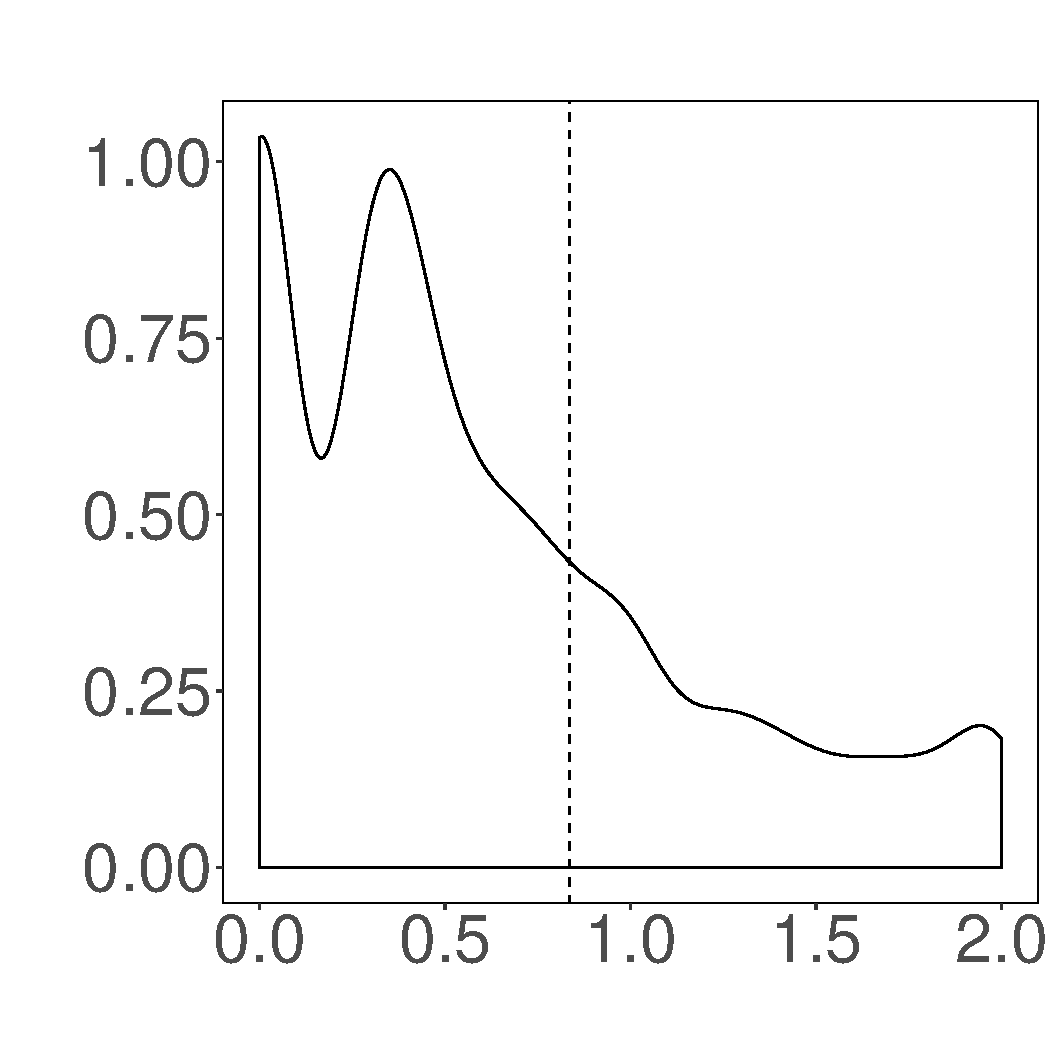
\includegraphics[width=\linewidth]{Figures/mem-cassandra-cluster.pdf}
                \caption{Memory}
        \end{subfigure}%
        \begin{subfigure}{0.19\textwidth}
                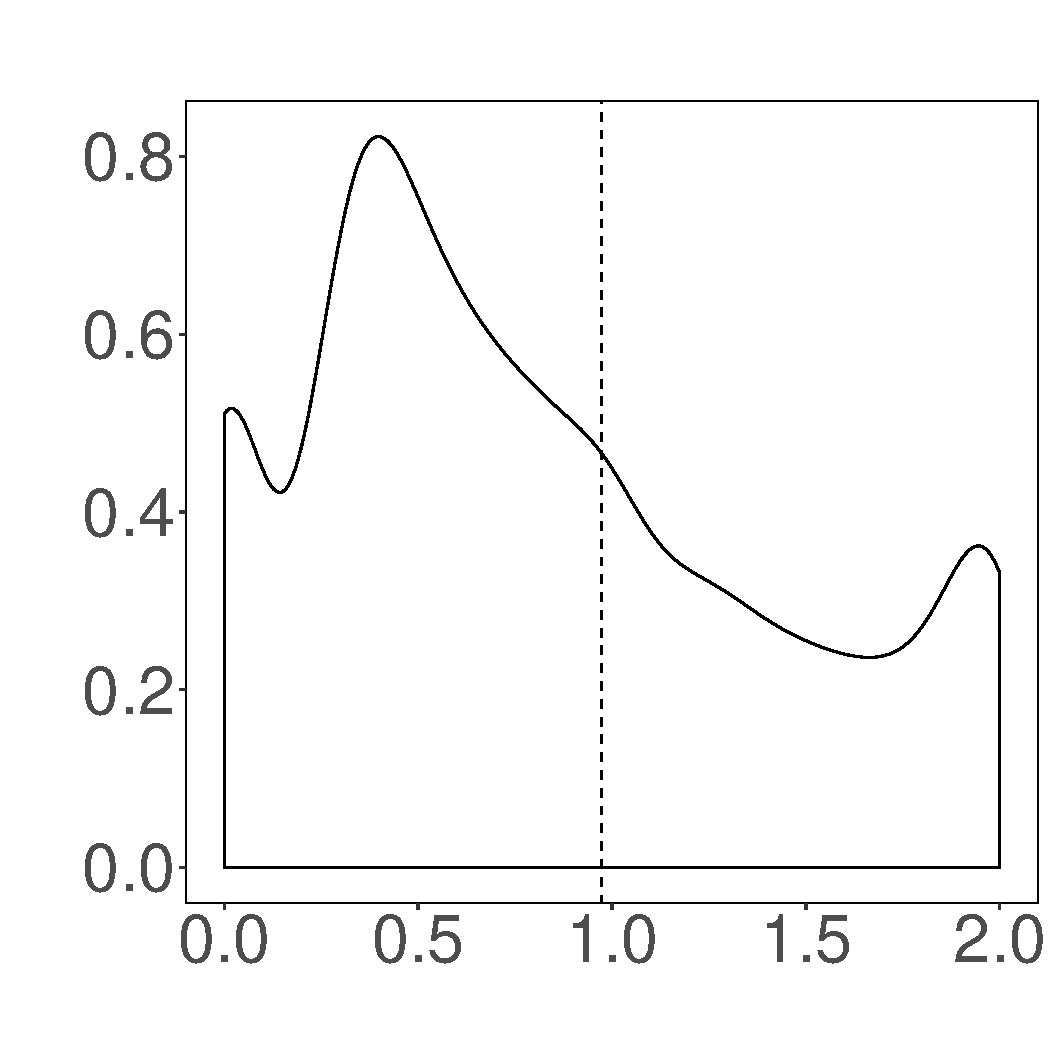
\includegraphics[width=\linewidth]{Figures/ioread-cassandra-cluster.pdf}
                \caption{I/O read}
        \end{subfigure}
        \begin{subfigure}{0.19\textwidth}
                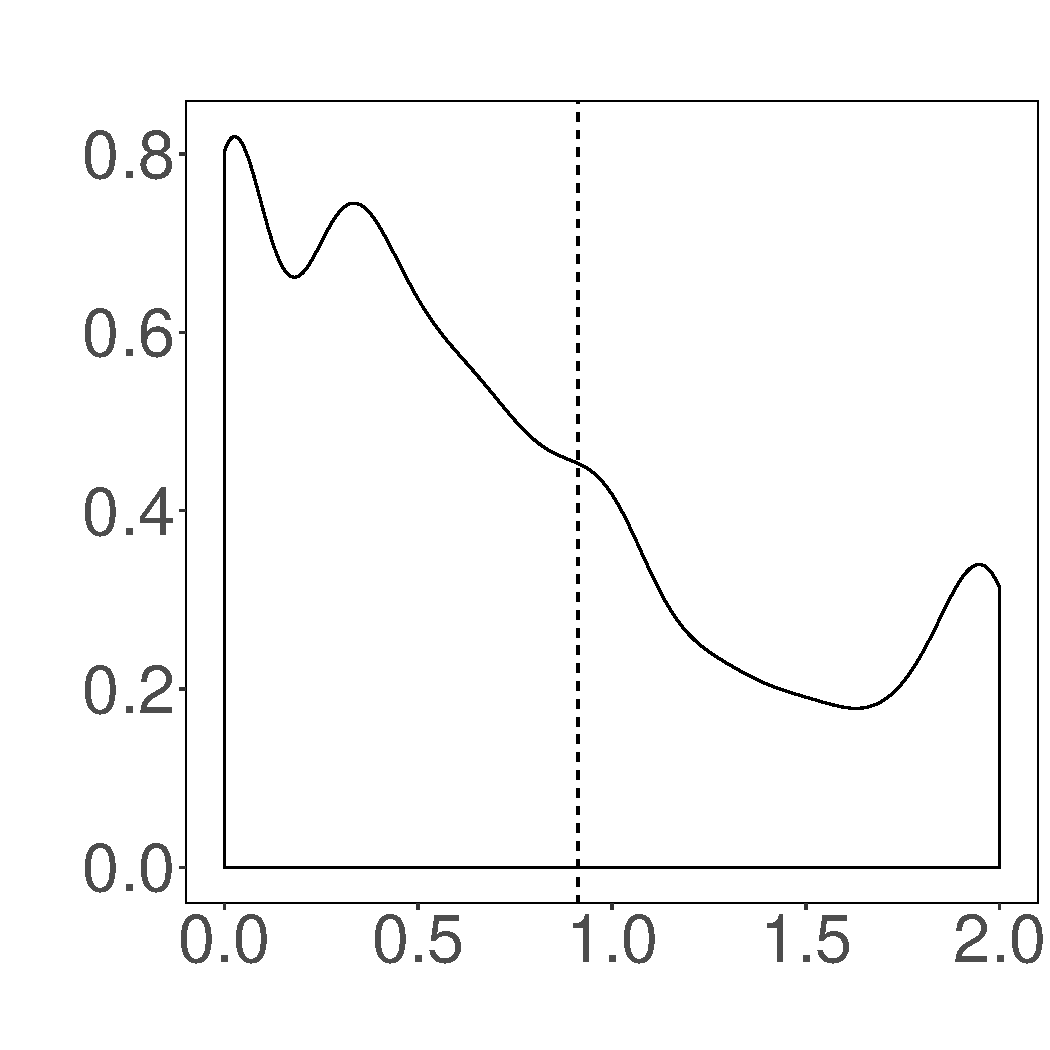
\includegraphics[width=\linewidth]{Figures/iowrite-cassandra-cluster.pdf}
                \caption{I/O write}
        \end{subfigure}
        
	\caption{The automatically obtained thresholds for splitting option variation into \inconsistent and non-\inconsistent groups for \emph{Cassandra}.} % \med{Canssadra or Hadoop? Both fig. 3 and fig. 4 showed Hadoop}.}
	\label{fig:threshold_cassandra}
% 	\vspace{-0.15cm}
\end{figure}


%%% Local Variables:
%%% mode: latex
%%% TeX-master: "../main"
%%% End:
